% MICRO 2026 Survey Paper - ML Performance Models
% Using MICRO 59 ACM sigconf template

%%
%% For submission and review of your manuscript please change the
%% command to \documentclass[manuscript, screen, review]{acmart}.
%%
\documentclass[sigconf, screen, review]{acmart}

%%
%% \BibTeX command to typeset BibTeX logo in the docs
\AtBeginDocument{%
  \providecommand\BibTeX{{%
    Bib\TeX}}}

%% Rights management information - for submission
\setcopyright{none}
\copyrightyear{2026}
\acmYear{2026}
\acmDOI{XXXXXXX.XXXXXXX}

%% Conference information
\acmConference[MICRO 2026]{The 59th IEEE/ACM International Symposium on Microarchitecture}{November 2026}{Austin, TX, USA}
\acmISBN{978-X-XXXX-XXXX-X/XX/XX}

%% Disable ACM reference format printing for submission
\settopmatter{printfolios=true}
\settopmatter{printacmref=false}

%% Additional packages (acmart already loads amsmath, amsfonts, amssymb, booktabs)
\usepackage{multirow}
\usepackage{tikz}
\usetikzlibrary{shapes.geometric,arrows.meta,positioning,fit,backgrounds}

% Custom commands
\newcommand{\todo}[1]{\textcolor{red}{[TODO: #1]}}

\begin{document}

\title{A Survey of High-Level Modeling and Simulation Methods for Modern Machine Learning Workloads}
\subtitle{\normalsize{MICRO 2026 Submission
    \textbf{\#NaN} -- Confidential Draft -- Do NOT Distribute!!}}

%%
%% The abstract is a short summary of the work to be presented in the
%% article.

%%%%%% -- PAPER CONTENT STARTS-- %%%%%%%%

\begin{abstract}
Machine learning-based performance modeling has emerged as a powerful alternative to traditional analytical models and cycle-accurate simulators for predicting computer system behavior.
This survey focuses specifically on \emph{ML techniques} for performance prediction across CPUs, GPUs, accelerators, and distributed systems, covering over 60 papers from architecture and ML venues published between 2016--2025.
We position traditional analytical models (Timeloop, MAESTRO) and simulators (gem5, GPGPU-Sim) as \emph{baselines} that ML approaches aim to replace or augment.
We organize ML approaches along three primary dimensions---modeling technique, target hardware, and input representation---while additionally characterizing papers by workload coverage, prediction targets, accuracy metrics, and evaluation scope.
Our analysis reveals that specialized ML models achieve remarkable accuracy---below 5\% error for narrow domains---while general-purpose models trade accuracy for broader applicability.
Transfer learning and meta-learning techniques increasingly enable adaptation to new hardware with minimal profiling, addressing the challenge of hardware diversity.
We identify key open challenges including benchmark diversity, cross-platform generalization, and integration with compiler and architecture exploration workflows.
Hybrid approaches combining analytical structure with learned components represent the most promising direction, offering both interpretability and accuracy.
This survey provides practitioners guidance for selecting appropriate ML techniques and researchers a roadmap for advancing the field.
\end{abstract}

%%
%% Keywords
\keywords{machine learning, performance modeling, computer architecture, neural networks, survey}

\maketitle

% ==============================================================================
% INTRODUCTION
% ==============================================================================
\section{Introduction}
\label{sec:introduction}

Performance modeling is fundamental to computer architecture research and development.
Architects rely on accurate performance predictions to navigate vast design spaces, optimize hardware-software co-design, and make informed decisions about resource allocation.
Traditional approaches---analytical models~\cite{williams2009roofline} and cycle-accurate simulators~\cite{binkert2011gem5}---have served the community well, but face growing challenges as workloads and hardware become increasingly complex.
Analytical models often oversimplify system behavior, while simulators can require hours or days to evaluate a single design point, making exhaustive exploration impractical.

The rise of deep learning workloads has intensified these challenges.
Modern neural networks exhibit diverse computational patterns---from dense matrix operations in transformers to sparse irregular accesses in graph neural networks---that stress traditional modeling assumptions.
Simultaneously, hardware diversity has exploded: GPUs, TPUs, custom accelerators, and multi-device distributed systems each present unique performance characteristics that resist unified analytical treatment.
This complexity has motivated a new generation of \emph{machine learning-based} performance models that learn predictive functions directly from profiling data.

ML-based performance modeling has emerged as a compelling alternative.
Learned models can capture complex, non-linear relationships between workload characteristics and hardware behavior that elude closed-form analysis.
Recent work demonstrates remarkable accuracy: NeuSight~\cite{neusight2025} achieves 2.3\% error predicting GPT-3 latency on H100 GPUs, while nn-Meter~\cite{nnmeter2021} reaches 99\% accuracy for edge device latency prediction.
Beyond accuracy, these approaches offer practical benefits: models trained on one platform can transfer to new hardware with minimal adaptation~\cite{litepred2024}, and inference-time predictions complete in milliseconds rather than hours.

This survey provides a comprehensive analysis of ML-based performance modeling techniques for computer architecture.
We focus specifically on \emph{learned} models that acquire predictive capability from data, positioning traditional analytical and simulation approaches as baselines that contextualize ML advances.
We make the following contributions:
\begin{itemize}
    \item A \textbf{taxonomy} organizing ML approaches along three primary dimensions (modeling technique, target hardware, input representation), with additional characterization by workload coverage, prediction targets, and accuracy.
    \item A \textbf{systematic survey} of over 60 ML-based performance modeling papers from architecture venues (MICRO, ISCA, HPCA, ASPLOS) and ML venues (MLSys, NeurIPS, ICML) published between 2016--2025.
    \item A \textbf{comparative analysis} examining trade-offs between accuracy, training cost, generalization, and interpretability across ML approaches.
    \item An identification of \textbf{open challenges} including data scarcity, cross-platform generalization, and integration with design automation flows.
\end{itemize}

The remainder of this paper is organized as follows.
Section~\ref{sec:background} provides background on traditional performance modeling and relevant ML techniques.
Section~\ref{sec:taxonomy} presents our classification taxonomy.
Section~\ref{sec:survey} surveys approaches organized by target hardware platform.
Section~\ref{sec:comparison} offers comparative analysis across key dimensions.
Section~\ref{sec:challenges} discusses open challenges and future directions.
Section~\ref{sec:evaluation} presents hands-on reproducibility evaluations of representative tools.
Section~\ref{sec:conclusion} concludes.

Figure~\ref{fig:timeline} illustrates the evolution of ML-based performance modeling, showing how techniques have progressed from simple regression models to sophisticated hybrid approaches achieving sub-5\% accuracy.

\begin{figure}[t]
\centering
\resizebox{\columnwidth}{!}{%
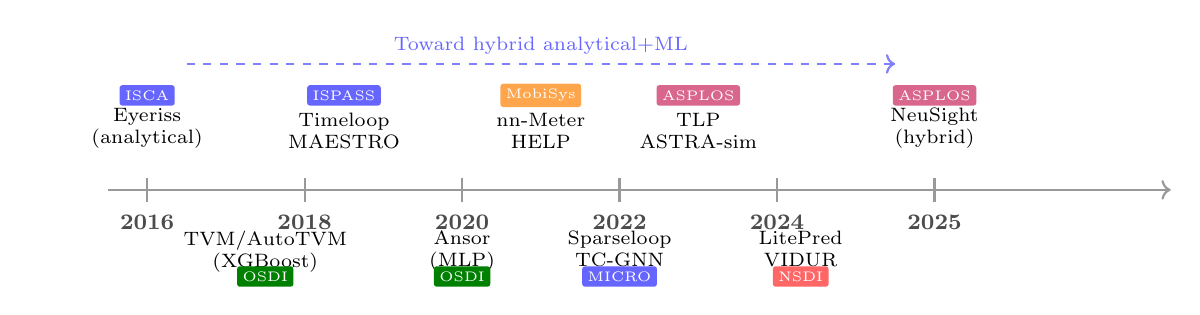
\begin{tikzpicture}[
    node distance=0.3cm,
    yearnode/.style={font=\footnotesize\bfseries, text=black!70},
    eventnode/.style={font=\scriptsize, text width=2.8cm, align=center},
    catnode/.style={font=\tiny, text=white, rounded corners=1pt, inner sep=2pt}
]
% Timeline base
\draw[thick, ->, black!40] (0,0) -- (13.5,0);

% Year markers
\foreach \x/\year in {0.5/2016, 2.5/2018, 4.5/2020, 6.5/2022, 8.5/2024, 10.5/2025} {
    \draw[thick, black!40] (\x,-0.15) -- (\x,0.15);
    \node[yearnode, below] at (\x,-0.2) {\year};
}

% Events - staggered heights to avoid overlap
% 2016-2017: Foundation
\node[eventnode, above] at (0.5,0.4) {Eyeriss\\(analytical)};
\node[catnode, fill=blue!60] at (0.5,1.2) {ISCA};

% 2018: TVM
\node[eventnode, below] at (2.0,-0.4) {TVM/AutoTVM\\(XGBoost)};
\node[catnode, fill=green!50!black] at (2.0,-1.1) {OSDI};

% 2019: Timeloop, MAESTRO
\node[eventnode, above] at (3.0,0.4) {Timeloop\\MAESTRO};
\node[catnode, fill=blue!60] at (3.0,1.2) {ISPASS};

% 2020: Ansor
\node[eventnode, below] at (4.5,-0.4) {Ansor\\(MLP)};
\node[catnode, fill=green!50!black] at (4.5,-1.1) {OSDI};

% 2021: nn-Meter, HELP
\node[eventnode, above] at (5.5,0.4) {nn-Meter\\HELP};
\node[catnode, fill=orange!70] at (5.5,1.2) {MobiSys};

% 2022: Sparseloop, GNN
\node[eventnode, below] at (6.5,-0.4) {Sparseloop\\TC-GNN};
\node[catnode, fill=blue!60] at (6.5,-1.1) {MICRO};

% 2023: TLP, ASTRA-sim
\node[eventnode, above] at (7.5,0.4) {TLP\\ASTRA-sim};
\node[catnode, fill=purple!60] at (7.5,1.2) {ASPLOS};

% 2024: LitePred, VIDUR
\node[eventnode, below] at (8.8,-0.4) {LitePred\\VIDUR};
\node[catnode, fill=red!60] at (8.8,-1.1) {NSDI};

% 2025: NeuSight
\node[eventnode, above] at (10.5,0.4) {NeuSight\\(hybrid)};
\node[catnode, fill=purple!60] at (10.5,1.2) {ASPLOS};

% Trend arrow
\draw[thick, ->, blue!50, dashed] (1,1.6) -- (10,1.6);
\node[font=\scriptsize, text=blue!60, above] at (5.5,1.6) {Toward hybrid analytical+ML};

\end{tikzpicture}
}
\caption{Evolution of ML-based performance modeling (2016--2025). Early work used analytical models (Eyeriss, Timeloop); ML approaches began with simple regressors (TVM) and progressed to deep learning (Ansor, HELP), GNNs (TC-GNN), and transformers (TLP). Current state-of-the-art combines analytical structure with neural networks (NeuSight).}
\label{fig:timeline}
\end{figure}

% ==============================================================================
% BACKGROUND
% ==============================================================================
\section{Background}
\label{sec:background}

\subsection{Traditional Performance Modeling}
\label{subsec:traditional-modeling}

Before ML-based approaches, performance modeling relied on two complementary paradigms: analytical models and cycle-accurate simulation.
This section reviews both as \emph{baselines} against which ML techniques are compared, identifying their limitations that motivate learned alternatives.

\subsubsection{Analytical Models}

Analytical models express performance as closed-form functions of hardware and workload parameters.
The roofline model~\cite{williams2009roofline} exemplifies this approach, bounding attainable performance by peak compute throughput and memory bandwidth.
Given operational intensity $I$ (FLOP/byte), the roofline predicts performance as $P = \min(\pi, \beta \cdot I)$, where $\pi$ is peak FLOPS and $\beta$ is memory bandwidth.
Despite its simplicity, roofline reasoning guides optimization by revealing compute-bound versus memory-bound regimes.

For DNN accelerators, analytical cost models have become standard practice.
Timeloop~\cite{timeloop2019} models data movement across memory hierarchies for any given mapping (loop order and tiling), computing access counts and energy from architectural parameters.
MAESTRO~\cite{maestro2019} provides a data-centric framework that derives performance from dataflow descriptions.
Sparseloop~\cite{sparseloop2022} extends this methodology to sparse tensor operations, achieving 2000$\times$ speedup over RTL simulation while maintaining accuracy.

Analytical models offer several advantages: fast evaluation (microseconds per design point), interpretability (designers can trace predictions to specific terms), and extrapolation to unseen configurations.
However, they require manual derivation for each target architecture, struggle to capture complex microarchitectural effects (contention, pipeline stalls, caching behavior), and may oversimplify non-linear interactions.

\subsubsection{Cycle-Accurate Simulation}

Cycle-accurate simulators model hardware at register-transfer level, faithfully reproducing timing behavior.
General-purpose simulators like gem5~\cite{binkert2011gem5} support flexible configuration of CPU cores, caches, memory controllers, and interconnects.
For GPUs, simulators such as GPGPU-Sim~\cite{gpgpusim2009} and Accel-Sim~\cite{accelsim2020} model SIMT execution, warp scheduling, and memory coalescing.

Cycle-accurate simulation achieves high fidelity---typically within 5--15\% of real hardware~\cite{binkert2011gem5}---and supports detailed microarchitectural studies.
However, simulation speed presents a fundamental limitation: evaluating a single ResNet-50 inference may require hours, making design space exploration impractical.
ASTRA-sim~\cite{astrasim2023} addresses distributed training at scale through analytical abstractions, but even coarse-grained simulation struggles with the combinatorial explosion of modern ML workloads and hardware configurations.

\subsubsection{The Modeling Gap}

Neither approach fully addresses modern performance modeling needs.
Analytical models are fast but imprecise for complex microarchitectures.
Simulators are accurate but too slow for iterative design.
This tension has intensified as ML workloads diversify (from CNNs to transformers to mixture-of-experts models) and hardware specializes (GPUs, TPUs, custom accelerators).
ML-based performance models offer a middle path: learning complex relationships from profiling data while enabling millisecond-scale inference.

\subsection{Machine Learning Fundamentals}
\label{subsec:ml-fundamentals}

This section provides a brief primer on ML techniques frequently employed in performance modeling, establishing terminology used throughout the survey.

\subsubsection{Classical Machine Learning}

Linear regression and its regularized variants (ridge, LASSO) remain widely used for performance prediction due to their simplicity and interpretability.
Given feature vector $\mathbf{x}$ (e.g., operator parameters, hardware counters), linear models predict $\hat{y} = \mathbf{w}^\top \mathbf{x} + b$.
While unable to capture non-linear relationships, linear models provide baselines and feature importance rankings.

Tree-based ensembles---random forests and gradient boosted trees (XGBoost, LightGBM)---handle non-linearities through recursive partitioning.
These methods dominate when training data is limited ($<$10K samples) and features are well-engineered, often outperforming deep learning in low-data regimes~\cite{nnmeter2021}.

\subsubsection{Deep Learning}

Multi-layer perceptrons (MLPs) learn hierarchical feature representations through stacked non-linear transformations: $\mathbf{h}_{i+1} = \sigma(\mathbf{W}_i \mathbf{h}_i + \mathbf{b}_i)$.
MLPs require minimal feature engineering but need sufficient training data and careful regularization to avoid overfitting.

Recurrent neural networks (RNNs) and their gated variants (LSTM, GRU) process sequential inputs, making them suitable for modeling operator sequences in neural network execution graphs.
However, sequential processing limits parallelization and can miss long-range dependencies.

\subsubsection{Graph Neural Networks}

Graph neural networks (GNNs) operate on graph-structured data through message passing.
For a node $v$ with features $\mathbf{h}_v$, GNNs iteratively update representations by aggregating information from neighbors $\mathcal{N}(v)$:
\begin{equation}
\mathbf{h}_v^{(k+1)} = \phi\left(\mathbf{h}_v^{(k)}, \bigoplus_{u \in \mathcal{N}(v)} \psi(\mathbf{h}_u^{(k)}, \mathbf{e}_{uv})\right)
\end{equation}
where $\phi$ and $\psi$ are learnable functions and $\oplus$ is a permutation-invariant aggregation (sum, mean, max).

GNNs are particularly appealing for performance modeling because DNN computation graphs have natural graph structure.
Nodes represent operators with features (type, parameters), edges represent data dependencies with features (tensor shapes, datatypes).
GNNs can learn to propagate performance-relevant information along these dependencies~\cite{granite2022}.

\subsubsection{Attention and Transformers}

Attention mechanisms compute weighted combinations over input elements, with weights determined by learned compatibility functions.
Self-attention allows each position to attend to all other positions:
\begin{equation}
\text{Attention}(\mathbf{Q}, \mathbf{K}, \mathbf{V}) = \text{softmax}\left(\frac{\mathbf{Q}\mathbf{K}^\top}{\sqrt{d_k}}\right)\mathbf{V}
\end{equation}

Transformers stack self-attention with feedforward networks, enabling long-range dependency modeling without sequential processing.
Recent performance models leverage transformer architectures to capture complex inter-operator interactions across entire computation graphs.

\subsubsection{Transfer Learning}

Transfer learning adapts models trained on one domain (source) to perform well on another (target).
In performance modeling, this enables training on easily-profiled hardware and transferring to new platforms with limited data.
Common approaches include fine-tuning (adjusting pre-trained weights with target data), domain adaptation (learning domain-invariant representations), and meta-learning (learning to adapt quickly from few examples)~\cite{litepred2024}.

\subsection{Problem Formulation}
\label{subsec:problem-formulation}

We now formally define the performance modeling problem and establish the evaluation framework used throughout this survey.

\subsubsection{Inputs and Outputs}

Performance modeling maps workload and hardware descriptions to performance metrics.
Formally, given workload specification $\mathcal{W}$ and hardware configuration $\mathcal{H}$, a performance model $f$ predicts metric $y$:
\begin{equation}
\hat{y} = f(\mathcal{W}, \mathcal{H}; \theta)
\end{equation}
where $\theta$ represents model parameters (weights for ML models, equations for analytical models).

\textbf{Workload representations} vary by granularity and abstraction:
\begin{itemize}
    \item \emph{Operator-level}: Individual layer parameters (kernel size, channels, batch size)
    \item \emph{Graph-level}: Full computation graph with node and edge features
    \item \emph{IR-level}: Intermediate representations from compilers (TVM~\cite{tvm2018}, XLA)
    \item \emph{Trace-level}: Execution traces capturing runtime behavior
\end{itemize}

\textbf{Hardware representations} similarly span multiple levels:
\begin{itemize}
    \item \emph{Specification}: Static parameters (core count, memory size, bandwidth)
    \item \emph{Counter-based}: Runtime performance counters (cache misses, stalls)
    \item \emph{Embedding}: Learned dense representations of hardware platforms
\end{itemize}

\subsubsection{Prediction Targets}

Performance models target various metrics depending on application requirements:

\textbf{Latency} measures execution time, typically end-to-end inference time or per-layer latency.
Latency prediction is critical for real-time applications with strict deadlines and for optimizing user-facing services.

\textbf{Throughput} captures sustained processing rate: samples per second for inference, tokens per second for language models, or images per second for training.
Throughput optimization maximizes hardware utilization for batch processing.

\textbf{Energy} encompasses power consumption (Watts) and energy per operation (Joules/inference).
Energy prediction is essential for mobile deployment, data center cost optimization, and sustainability considerations.

\textbf{Memory} includes peak memory footprint (for feasibility checking), memory bandwidth utilization, and memory access patterns.

\textbf{Multi-objective} formulations jointly predict multiple metrics, enabling Pareto-optimal design selection balancing latency, energy, and accuracy.

\subsubsection{Accuracy Metrics}

The field employs several accuracy metrics, each with distinct interpretations:

\textbf{Mean Absolute Percentage Error (MAPE)} measures average relative deviation:
\begin{equation}
\text{MAPE} = \frac{100\%}{n} \sum_{i=1}^{n} \left| \frac{y_i - \hat{y}_i}{y_i} \right|
\end{equation}
MAPE is scale-invariant and interpretable (5\% MAPE means predictions typically differ by 5\% from ground truth).

\textbf{Root Mean Square Error (RMSE)} penalizes large errors more heavily:
\begin{equation}
\text{RMSE} = \sqrt{\frac{1}{n} \sum_{i=1}^{n} (y_i - \hat{y}_i)^2}
\end{equation}

\textbf{Correlation coefficients} (Pearson, Spearman) measure how well predictions track relative ordering---important when models guide design space exploration.

\textbf{Ranking accuracy} directly evaluates whether models correctly order configurations, often measured via Kendall's $\tau$ or top-$k$ accuracy.

\subsubsection{Hardware Targets}

Modern performance modeling spans diverse hardware platforms:

\textbf{CPUs} remain important for general-purpose inference and training of smaller models.
CPU modeling must account for complex cache hierarchies, branch prediction, out-of-order execution, and SIMD vectorization.

\textbf{GPUs} dominate ML training and large-scale inference.
GPU modeling addresses SIMT execution, warp scheduling, memory coalescing, and multi-GPU scaling.

\textbf{TPUs and custom accelerators} employ specialized dataflows for matrix operations.
Modeling these devices requires understanding systolic arrays, on-chip memory hierarchies, and dataflow mappings.

\textbf{Edge devices} (mobile SoCs, embedded NPUs) impose strict power and memory constraints.
Edge modeling emphasizes latency under thermal throttling and memory-limited execution.

\textbf{Distributed systems} scale training across multiple devices and nodes.
Distributed modeling must capture communication overhead, synchronization barriers, and pipeline parallelism.

This diversity of targets, workloads, and metrics motivates our comprehensive taxonomy in Section~\ref{sec:taxonomy}.

% ==============================================================================
% TAXONOMY
% ==============================================================================
\section{Taxonomy}
\label{sec:taxonomy}

We organize the surveyed literature along three primary dimensions: the hardware target being modeled, the machine learning techniques employed, and the input representations used.
Figure~\ref{fig:taxonomy-overview} illustrates how these dimensions intersect to characterize different performance modeling approaches.
This taxonomy extends existing classifications~\cite{timeloop2019,maestro2019} by incorporating the emerging diversity of ML-based methods and their distinctive design choices.

Our classification scheme serves two purposes.
First, it provides a systematic framework for understanding the design space of ML-based performance models---researchers can identify which combinations of targets, techniques, and representations have been explored versus those that remain open.
Second, it enables practitioners to select appropriate methods for their use cases by matching problem characteristics (target hardware, available data, accuracy requirements) to model capabilities.

\begin{figure}[t]
\centering
\resizebox{\columnwidth}{!}{%
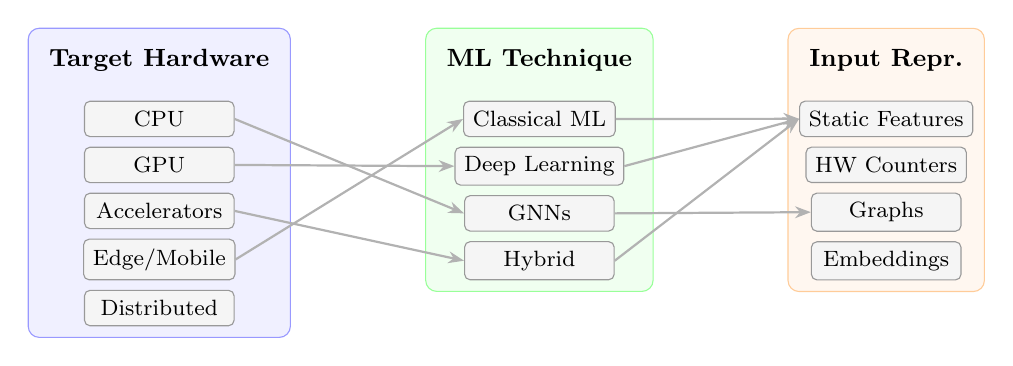
\begin{tikzpicture}[
    node distance=0.4cm and 0.6cm,
    dimbox/.style={rectangle, draw=black!70, fill=white, thick, minimum width=2.2cm, minimum height=0.6cm, font=\small},
    catbox/.style={rectangle, rounded corners=2pt, draw=black!40, fill=gray!8, minimum width=1.9cm, minimum height=0.45cm, font=\footnotesize},
    dimlabel/.style={font=\small\bfseries, text=black},
    arrow/.style={-{Stealth[length=2mm]}, thick, draw=black!50}
]

% === TARGET HARDWARE (Left column) ===
\node[dimlabel] (hw-label) at (0, 0) {Target Hardware};
\node[catbox, below=0.25cm of hw-label] (cpu) {CPU};
\node[catbox, below=0.12cm of cpu] (gpu) {GPU};
\node[catbox, below=0.12cm of gpu] (accel) {Accelerators};
\node[catbox, below=0.12cm of accel] (edge) {Edge/Mobile};
\node[catbox, below=0.12cm of edge] (dist) {Distributed};

% === ML TECHNIQUE (Middle column) ===
\node[dimlabel, right=2.0cm of hw-label] (ml-label) {ML Technique};
\node[catbox, below=0.25cm of ml-label] (classical) {Classical ML};
\node[catbox, below=0.12cm of classical] (deep) {Deep Learning};
\node[catbox, below=0.12cm of deep] (gnn) {GNNs};
\node[catbox, below=0.12cm of gnn] (hybrid) {Hybrid};

% === INPUT REPRESENTATION (Right column) ===
\node[dimlabel, right=2.0cm of ml-label] (inp-label) {Input Repr.};
\node[catbox, below=0.25cm of inp-label] (static) {Static Features};
\node[catbox, below=0.12cm of static] (counters) {HW Counters};
\node[catbox, below=0.12cm of counters] (graph) {Graphs};
\node[catbox, below=0.12cm of graph] (embed) {Embeddings};

% === Connecting arrows showing cross-dimensional relationships ===
% GPU -> Deep Learning (NeuSight, Habitat)
\draw[arrow, black!30] (gpu.east) -- (deep.west);
% Accelerators -> Hybrid (Timeloop, ArchGym)
\draw[arrow, black!30] (accel.east) -- (hybrid.west);
% Edge -> Classical ML (nn-Meter)
\draw[arrow, black!30] (edge.east) -- (classical.west);
% CPU -> GNN (GRANITE)
\draw[arrow, black!30] (cpu.east) -- (gnn.west);

% Deep Learning -> Static Features
\draw[arrow, black!30] (deep.east) -- (static.west);
% GNN -> Graph repr
\draw[arrow, black!30] (gnn.east) -- (graph.west);
% Classical ML -> Static/Counters
\draw[arrow, black!30] (classical.east) -- (static.west);
% Hybrid -> multiple
\draw[arrow, black!30] (hybrid.east) -- (static.west);

% === Background boxes for each dimension ===
\begin{scope}[on background layer]
    \node[fit=(hw-label)(cpu)(gpu)(accel)(edge)(dist), fill=blue!6, draw=blue!40, rounded corners=4pt, inner sep=4pt] {};
    \node[fit=(ml-label)(classical)(deep)(gnn)(hybrid), fill=green!6, draw=green!40, rounded corners=4pt, inner sep=4pt] {};
    \node[fit=(inp-label)(static)(counters)(graph)(embed), fill=orange!6, draw=orange!40, rounded corners=4pt, inner sep=4pt] {};
\end{scope}

\end{tikzpicture}%
}
\caption{Three-dimensional taxonomy for ML-based performance modeling. Arrows indicate common pairings observed in the literature (e.g., GPU models often use deep learning with static features).}
\label{fig:taxonomy-overview}
\end{figure}

\subsection{By Modeling Target}
\label{subsec:by-target}

The choice of hardware target fundamentally shapes model design, as different platforms exhibit distinct performance characteristics and modeling challenges.

\subsubsection{CPU Performance Modeling}

CPUs present complex modeling challenges due to deep out-of-order pipelines, sophisticated cache hierarchies, and branch prediction.
ML models for CPU performance must capture instruction-level parallelism, cache behavior, and memory access patterns.
Traditional approaches relied on microbenchmark-based linear regression~\cite{binkert2011gem5}, while recent work employs graph neural networks to model basic block throughput~\cite{granite2022}.
CPU modeling remains challenging due to the diversity of microarchitectures and the difficulty of capturing dynamic effects like branch misprediction and cache contention.

\subsubsection{GPU Performance Modeling}

GPUs dominate modern ML training and inference, making accurate GPU performance prediction critical.
GPU modeling must account for SIMT execution, warp scheduling, memory coalescing, and memory bandwidth limitations.
Early approaches used analytical roofline models~\cite{williams2009roofline}, but these struggle with the complex memory hierarchies and occupancy effects of modern GPUs.

ML-based GPU models have achieved remarkable accuracy.
NeuSight~\cite{neusight2025} introduces tile-based prediction that mirrors CUDA's execution model, achieving 2.3\% error on GPT-3 inference across H100, A100, and V100 GPUs.
Habitat~\cite{habitat2021} pioneered runtime-based cross-GPU prediction using wave scaling analysis.
These approaches demonstrate that learned models can capture GPU performance characteristics that elude analytical treatment.

\subsubsection{DNN Accelerator Modeling}

Custom DNN accelerators---including TPUs, NPUs, and systolic array designs---employ specialized dataflows optimized for matrix operations.
Modeling these devices requires understanding the interaction between dataflow, memory hierarchy, and tensor tiling.

Analytical frameworks like Timeloop~\cite{timeloop2019} and MAESTRO~\cite{maestro2019} provide systematic approaches for accelerator design space exploration.
Timeloop models data movement and compute utilization for any valid mapping of operations to hardware, achieving 5--10\% accuracy versus RTL simulation at 2000$\times$ speedup.
MAESTRO offers a data-centric perspective using intuitive dataflow directives.
Sparseloop~\cite{sparseloop2022} extends these frameworks to sparse tensor operations, critical for efficient transformer inference.

ML-based approaches complement analytical models by learning residual corrections or capturing effects not modeled analytically.
ArchGym~\cite{archgym2023} demonstrates that ML surrogate models can achieve 0.61\% RMSE while providing 2000$\times$ speedup over simulation, enabling rapid design space exploration for accelerator development.

\subsubsection{Edge and Mobile Device Modeling}

Edge devices impose strict power, memory, and latency constraints, making accurate prediction essential for deploying ML models on mobile phones, IoT devices, and embedded systems.
The diversity of edge hardware---spanning mobile CPUs, mobile GPUs, NPUs, and DSPs---creates significant challenges for cross-platform prediction.

nn-Meter~\cite{nnmeter2021} addresses this challenge through kernel-level prediction with adaptive sampling, achieving 99\% accuracy across mobile CPUs, GPUs, and Intel VPUs.
LitePred~\cite{litepred2024} extends this work with transfer learning, achieving 99.3\% accuracy across 85 edge platforms with less than one hour of adaptation per new device.
These results demonstrate that ML models can effectively generalize across the heterogeneous edge hardware landscape.

\subsubsection{Distributed System Modeling}

Multi-GPU and multi-node systems introduce communication overhead, synchronization barriers, and parallelism strategy choices that fundamentally change performance characteristics.
Distributed training performance depends on the interplay between compute, memory bandwidth, and network communication.

ASTRA-sim~\cite{astrasim2023} provides end-to-end distributed training simulation, modeling collective communication algorithms, network topology, and compute-communication overlap.
VIDUR~\cite{vidur2024} focuses specifically on LLM inference serving, capturing the unique characteristics of prefill and decode phases, KV cache management, and request scheduling.
These simulation frameworks achieve 5--15\% accuracy versus real clusters while enabling exploration of parallelization strategies at scale.

\subsection{By ML Technique}
\label{subsec:by-technique}

The choice of ML technique reflects trade-offs between accuracy, data efficiency, interpretability, and generalization capability.

\subsubsection{Classical Machine Learning}

Tree-based ensembles---random forests and gradient boosted trees (XGBoost, LightGBM)---remain highly effective for performance modeling, particularly in low-data regimes.
These methods handle non-linear relationships through recursive partitioning, provide feature importance rankings for interpretability, and require minimal hyperparameter tuning.

Classical ML models dominate when training data is limited ($<$10K samples) or when features are well-engineered.
nn-Meter~\cite{nnmeter2021} demonstrates that random forests achieve competitive accuracy with careful kernel-level feature engineering.
The ALCOP framework combines XGBoost with analytical pre-training, using analytical model predictions as features to accelerate autotuning convergence.

\subsubsection{Deep Learning}

Multi-layer perceptrons (MLPs) learn hierarchical feature representations without manual feature engineering.
MLPs are widely used as the prediction head in more complex architectures and as standalone models when sufficient training data is available.
NeuSight~\cite{neusight2025} uses MLPs to predict tile-level GPU utilization, learning complex interactions between tile parameters and hardware characteristics.

Recurrent neural networks (RNNs and LSTMs) process sequential inputs, making them suitable for modeling operator sequences in neural network execution.
However, sequential processing limits parallelization, and attention-based architectures increasingly replace RNNs for sequence modeling tasks.

\subsubsection{Graph Neural Networks}

Graph neural networks (GNNs) have emerged as particularly effective for performance modeling because computational graphs have natural graph structure.
Nodes represent operators with features (type, parameters, shapes), edges represent data dependencies with features (tensor dimensions, datatypes).
GNNs propagate performance-relevant information along these dependencies through message passing.

GRANITE~\cite{granite2022} applies GNNs to basic block throughput estimation, learning to predict CPU performance from instruction dependency graphs.
For DNN workloads, GNN-based models capture inter-operator interactions that flat feature representations miss.
The graph structure also enables natural handling of variable-size networks without padding or truncation.

\subsubsection{Hybrid Analytical+ML Models}

Hybrid approaches combine physics-based analytical models with learned components, achieving both interpretability and high accuracy.
The analytical component provides a strong prior based on hardware characteristics, while the ML component learns residual corrections and complex interactions.

This design philosophy has produced state-of-the-art results.
Analytical pre-training initializes ML models with reasonable predictions, reducing data requirements and improving convergence.
Physics-informed architectures incorporate analytical insights into model structure---NeuSight's tile-based prediction mirrors CUDA's execution model, providing inductive bias that improves generalization.
Residual learning trains ML models to predict the error of analytical models, combining analytical interpretability with ML's ability to capture unmodeled effects.

The latency predictor study~\cite{latencypredictorsnas2024} demonstrates that hybrid approaches with transfer learning achieve 22.5\% average improvement over baselines, with up to 87.6\% improvement on challenging cross-platform prediction tasks.

\subsection{By Input Representation}
\label{subsec:by-input}

Input representation determines what information the model can access and how effectively it can learn performance-relevant patterns.

\subsubsection{Static Features}

Static features derive from workload and hardware specifications without runtime measurement.
For DNN workloads, these include layer parameters (kernel size, channels, stride, batch size), tensor dimensions, and operator types.
Hardware specifications include core counts, memory sizes, bandwidth, and clock frequencies.

Static features enable prediction without profiling, supporting use cases like neural architecture search where thousands of candidate networks must be evaluated.
Feature engineering plays a critical role: effective representations capture computation-to-communication ratios, memory footprint estimates, and parallelization potential.

\subsubsection{Hardware Counters}

Performance counters provide runtime measurements of hardware behavior: cache miss rates, memory bandwidth utilization, instruction throughput, and stall cycles.
Counter-based models can capture dynamic effects invisible to static analysis, including contention, thermal throttling, and runtime scheduling decisions.

The primary limitation is that counter-based models require hardware execution, limiting their applicability for design space exploration or new architecture evaluation.
However, for optimizing existing deployments or debugging performance anomalies, counter-based models provide valuable insights that static approaches cannot match.

\subsubsection{Graph Representations}

Graph representations encode computational graphs with nodes representing operators and edges representing data dependencies.
Node features capture operator characteristics (type, parameters), while edge features encode tensor properties (shape, datatype, memory format).

Graph representations provide several advantages over flat feature vectors: they naturally handle variable-size networks, preserve structural information about operator interactions, and enable permutation-invariant predictions.
GNNs operating on these representations can learn which subgraph patterns indicate performance bottlenecks.

\subsubsection{Learned Embeddings}

Learned embeddings compress high-dimensional or categorical information into dense vector representations.
Hardware embeddings represent diverse devices as points in a learned feature space, enabling transfer learning across platforms.
Operator embeddings capture semantic similarities between operator types that may share performance characteristics.

HELP formulates hardware prediction as meta-learning, learning hardware embeddings that represent devices as black-box functions.
With just 10 measurement samples on a new device, HELP achieves accurate predictions by positioning the device appropriately in the learned embedding space.
This approach is particularly valuable for the fragmented edge hardware landscape, where collecting exhaustive training data for each device is impractical.

Table~\ref{tab:taxonomy-summary} summarizes representative papers across our taxonomy dimensions, illustrating the diversity of approaches and their key characteristics.

\begin{table*}[t]
\centering
\caption{Representative papers classified by our taxonomy dimensions. Accuracy reported as MAPE or correlation where available.}
\label{tab:taxonomy-summary}
\small
\begin{tabular}{llllll}
\toprule
\textbf{Paper} & \textbf{Target} & \textbf{Technique} & \textbf{Input} & \textbf{Accuracy} & \textbf{Key Contribution} \\
\midrule
NeuSight~\cite{neusight2025} & GPU & Hybrid & Static & 2.3\% & Tile-based prediction \\
nn-Meter~\cite{nnmeter2021} & Edge & Classical ML & Static & $<$5\% & Kernel detection \\
LitePred~\cite{litepred2024} & Edge & Transfer & Static & 0.7\% & 85-platform transfer \\
GRANITE~\cite{granite2022} & CPU & GNN & Graph & 0.97 corr & Basic block modeling \\
Timeloop~\cite{timeloop2019} & Accelerator & Analytical & Static & 5--10\% & Loop-nest DSE \\
ASTRA-sim~\cite{astrasim2023} & Distributed & Simulation & Traces & 5--15\% & Collective modeling \\
ArchGym~\cite{archgym2023} & Accelerator & Hybrid & Static & 0.61\% RMSE & ML-aided DSE \\
\bottomrule
\end{tabular}
\end{table*}

% ==============================================================================
% SURVEY OF APPROACHES
% ==============================================================================
\section{Survey of Approaches}
\label{sec:survey}

This section surveys ML-based performance modeling approaches organized by target hardware platform.
For each category, we examine the modeling challenges specific to that platform, describe representative techniques, and synthesize key findings across the literature.
Table~\ref{tab:survey-summary} provides a comprehensive comparison of the surveyed approaches.

\begin{table*}[t]
\centering
\caption{Summary of surveyed ML-based performance modeling approaches, organized by target hardware platform.}
\label{tab:survey-summary}
\small
\begin{tabular}{llllll}
\toprule
\textbf{Paper} & \textbf{Platform} & \textbf{ML Technique} & \textbf{Prediction Target} & \textbf{Error} & \textbf{Key Innovation} \\
\midrule
\multicolumn{6}{l}{\textit{CPU Performance Modeling}} \\
GRANITE~\cite{granite2022} & CPU & GNN & Basic block throughput & 0.97 corr & Instruction graph encoding \\
gem5+ML~\cite{binkert2011gem5} & CPU & Hybrid & Execution time & 10--20\% & Simulation + learning \\
\midrule
\multicolumn{6}{l}{\textit{GPU Performance Modeling}} \\
NeuSight~\cite{neusight2025} & GPU & Hybrid MLP & Kernel/E2E latency & 2.3\% & Tile-based prediction \\
Habitat~\cite{habitat2021} & GPU & MLP & Training time & 11.8\% & Wave scaling analysis \\
Accel-Sim~\cite{accelsim2020} & GPU & Simulation & Cycle-accurate & 10--20\% & SASS trace-driven \\
\midrule
\multicolumn{6}{l}{\textit{DNN Accelerator Modeling}} \\
Timeloop~\cite{timeloop2019} & NPU & Analytical & Latency/Energy & 5--10\% & Loop-nest DSE \\
MAESTRO~\cite{maestro2019} & NPU & Analytical & Latency/Energy & 5--15\% & Data-centric directives \\
Sparseloop~\cite{sparseloop2022} & NPU & Analytical & Sparse tensors & 5--10\% & Compression modeling \\
ArchGym~\cite{archgym2023} & Multi & RL+Surrogate & Multi-objective & 0.61\% & ML-aided DSE \\
\midrule
\multicolumn{6}{l}{\textit{Edge Device Modeling}} \\
nn-Meter~\cite{nnmeter2021} & Edge & RF ensemble & Latency & $<$1\% & Kernel detection \\
LitePred~\cite{litepred2024} & Edge & VAE+MLP & Latency & 0.7\% & 85-platform transfer \\
HELP~\cite{help2021} & Multi & Meta-learning & Latency & 1.9\% & 10-sample adaptation \\
\midrule
\multicolumn{6}{l}{\textit{Distributed and LLM Systems}} \\
ASTRA-sim~\cite{astrasim2023} & Distributed & Simulation & Training time & 5--15\% & Collective modeling \\
VIDUR~\cite{vidur2024} & GPU cluster & Simulation & LLM serving & $<$5\% & Prefill/decode phases \\
\bottomrule
\end{tabular}
\end{table*}

\subsection{CPU Performance Modeling}
\label{subsec:cpu-modeling}

CPU performance modeling for ML workloads presents unique challenges due to complex microarchitectural effects including out-of-order execution, branch prediction, and deep cache hierarchies.
While GPUs have received more attention for DNN training, CPUs remain important for inference---particularly on edge devices and for operators that map poorly to SIMT execution.

\subsubsection{Traditional CPU Performance Modeling}

Traditional CPU modeling relies on cycle-accurate simulation through frameworks like gem5~\cite{binkert2011gem5}.
The gem5 simulator provides multiple fidelity levels: fast functional simulation for correctness validation, and detailed out-of-order models achieving 10--20\% accuracy versus real hardware.
For ML workloads, gem5 extensions such as gem5-Aladdin and SMAUG enable accelerator integration studies.

However, cycle-accurate simulation suffers from fundamental speed limitations---simulating even modest DNN inference requires hours, making design space exploration impractical.
This limitation has motivated ML-based alternatives that learn to predict performance from static program features.

\subsubsection{ML-Based Basic Block Modeling}

GRANITE~\cite{granite2022} represents the state of the art in ML-based CPU performance modeling.
The key insight is that basic block throughput---the steady-state execution rate of a loop body---can be predicted from the instruction dependency graph without simulation.
GRANITE encodes basic blocks as directed graphs where nodes represent instructions with features (opcode, operand types) and edges capture data dependencies.

A graph neural network processes this representation through message passing layers:
\begin{equation}
\mathbf{h}_i^{(k+1)} = \text{MLP}\left(\mathbf{h}_i^{(k)} + \sum_{j \in \mathcal{N}(i)} \mathbf{h}_j^{(k)}\right)
\end{equation}
where $\mathbf{h}_i^{(k)}$ represents instruction $i$'s embedding at layer $k$.
After several message passing rounds, a global pooling operation aggregates instruction embeddings into a single block representation, which a final MLP maps to throughput prediction.

GRANITE achieves 0.97 Kendall's $\tau$ correlation with ground-truth measurements on x86 basic blocks, significantly outperforming prior analytical models like IACA and llvm-mca.
Critically, the learned model generalizes across microarchitectures---a model trained on Skylake transfers to Haswell with only modest accuracy degradation.

\subsubsection{Challenges and Opportunities}

Despite GRANITE's success, several challenges remain for CPU performance modeling.
First, DNN operators often involve memory-bound execution where cache behavior dominates---GRANITE focuses on compute-bound basic blocks and does not model memory hierarchy effects.
Second, modern CPUs feature increasingly complex prefetchers and branch predictors whose behavior is difficult to capture in static features.
Third, CPU-based DNN inference often involves highly optimized library code (Intel MKL, ARM Compute Library) whose performance depends on runtime scheduling decisions.

Hybrid approaches combining coarse-grained simulation with learned correction factors represent a promising direction.
Rather than simulating every cycle, these methods use fast simulation to establish approximate behavior, then train ML models to predict residual errors, potentially achieving simulation accuracy at reduced cost.

\subsection{GPU Performance Modeling}
\label{subsec:gpu-modeling}

GPUs are the dominant platform for ML training and large-scale inference.
Accurate GPU performance prediction is essential for neural architecture search, compiler optimization, and serving system design.
However, GPU performance modeling is challenging due to SIMT execution, complex memory hierarchies, and workload-dependent scheduling behavior.

\subsubsection{Cycle-Accurate GPU Simulation}

GPGPU-Sim~\cite{gpgpusim2009} pioneered detailed GPU simulation, modeling SIMT cores, warp scheduling, memory coalescing, and cache hierarchies.
Accel-Sim~\cite{accelsim2020} extended this foundation with trace-driven simulation and improved correlation with modern GPUs (Turing, Ampere), achieving 0.90--0.97 IPC correlation.

These simulators provide high fidelity---essential for microarchitectural studies---but suffer from 1000--10000$\times$ slowdown versus real GPU execution.
Simulating a single ResNet-50 inference can require hours, making design space exploration impractical.
This has motivated the development of ML-based predictors that achieve comparable accuracy at dramatically reduced cost.

\subsubsection{Learned GPU Performance Models}

Habitat~\cite{habitat2021} introduced \emph{wave scaling} for cross-GPU prediction.
The key insight is that GPU execution time can be decomposed into compute and memory components that scale differently across devices:
\begin{equation}
T_{\text{target}} = T_{\text{compute}} \cdot \frac{P_{\text{source}}}{P_{\text{target}}} + T_{\text{memory}} \cdot \frac{B_{\text{source}}}{B_{\text{target}}}
\end{equation}
where $P$ denotes peak compute throughput and $B$ memory bandwidth.
By profiling on a source GPU and measuring how kernels respond to artificially reduced parallelism (``wave scaling''), Habitat estimates the compute and memory fractions, enabling prediction on unseen target GPUs.

Habitat achieves 11.8\% average error predicting training iteration time across GPU generations (V100 to A100).
However, it requires actual GPU execution for wave scaling measurements and cannot predict performance for unseen models.

NeuSight~\cite{neusight2025} addresses these limitations through \emph{tile-based prediction}.
The key innovation is decomposing GPU kernel execution into tiles---the basic scheduling unit in CUDA---and predicting per-tile behavior:
\begin{equation}
T_{\text{kernel}} = \max_{w \in \text{waves}} \sum_{t \in w} \left( T_{\text{compute}}^{(t)} + T_{\text{memory}}^{(t)} \right)
\end{equation}

This formulation mirrors actual GPU execution semantics: tiles are scheduled in waves, and kernel time is dominated by the slowest wave.
NeuSight uses MLPs to predict tile-level compute and memory times from static features (tile dimensions, register usage, shared memory allocation).

By capturing the wave-level structure, NeuSight achieves remarkable accuracy: 2.3\% error on GPT-3 inference across H100, A100, and V100 GPUs.
This represents a 50$\times$ reduction in error compared to prior approaches like Habitat (121.4\% $\rightarrow$ 2.3\% on H100 for GPT-3).
NeuSight's physics-informed architecture---encoding GPU execution semantics into the model structure---provides strong inductive bias that enables generalization to unseen models and GPUs.

\subsubsection{Compiler Cost Models for GPUs}

The TVM~\cite{tvm2018} and Ansor~\cite{ansor2020} systems use learned cost models to guide tensor program optimization.
Rather than executing every candidate program, XGBoost or MLP models predict execution time from program features (loop bounds, vectorization widths, memory access patterns).

Ansor's hierarchical search combines sketch generation, random annotation, and evolutionary refinement, using the cost model to prune the search space.
With 10K profiled samples, Ansor achieves approximately 15\% MAPE on GPU kernel prediction.
The TenSet dataset provides 52 million program performance records across CPUs and GPUs, enabling pre-trained cost models that accelerate autotuning convergence by 10$\times$.

\subsubsection{LLM Inference Prediction}

Large language model inference presents unique GPU modeling challenges.
LLM execution exhibits distinct \emph{prefill} (compute-bound, parallel prompt processing) and \emph{decode} (memory-bound, sequential token generation) phases with fundamentally different performance characteristics.

VIDUR~\cite{vidur2024} provides discrete-event simulation for LLM serving systems.
Rather than modeling GPU microarchitecture, VIDUR simulates request scheduling, KV cache management, and batching decisions---the system-level factors that dominate serving performance.
VIDUR achieves $<$5\% error on end-to-end serving metrics including time-to-first-token and request latency.

Roofline-LLM extends traditional roofline analysis to LLM inference by decomposing transformer execution into compute-bound (prefill attention, FFN) and memory-bound (decode attention, KV cache access) components.
Combined with learned correction factors, this hybrid approach achieves 87\% reduction in MSE compared to pure roofline predictions.

\subsection{Accelerator Performance Modeling}
\label{subsec:accelerator-modeling}

DNN accelerators---including TPUs, NPUs, and custom ASIC designs---employ specialized dataflows and memory hierarchies optimized for tensor operations.
Modeling these devices requires understanding the interaction between dataflow choices, memory hierarchy utilization, and workload characteristics.

\subsubsection{Analytical Accelerator Modeling}

Timeloop~\cite{timeloop2019} provides the foundational framework for DNN accelerator design space exploration.
The key insight is that accelerator performance can be accurately predicted from loop-nest representations of tensor computations.
For a given architecture specification and mapping (loop order, tiling, spatial distribution), Timeloop analytically computes:

\begin{itemize}
\item \textbf{Data reuse} at each memory level: how many times each tensor element is accessed from each buffer
\item \textbf{Latency}: compute cycles plus memory stall cycles based on bandwidth constraints
\item \textbf{Energy}: access counts multiplied by per-access energy at each memory level
\end{itemize}

Timeloop decouples architecture specification (PEs, buffer sizes, bandwidth) from mapping decisions, enabling systematic exploration of dataflow choices.
The framework achieves 5--10\% accuracy versus RTL simulation while providing 2000$\times$ speedup, making million-point design sweeps tractable.

MAESTRO~\cite{maestro2019} offers a complementary \emph{data-centric} perspective.
Rather than loop-nest transformations, MAESTRO models performance through data movement analysis using compact dataflow directives.
This representation is more intuitive---designers specify how tensors flow through the architecture rather than manipulating loop indices---while achieving comparable accuracy.

Sparseloop~\cite{sparseloop2022} extends analytical modeling to sparse tensor accelerators.
The key challenge is that sparse execution time depends on runtime sparsity patterns, not just static tensor dimensions.
Sparseloop models compression formats (CSR, bitmap, RLE), gating logic, and sparse-dense conversion overhead, enabling accurate prediction for pruned neural networks and sparse attention patterns.

\subsubsection{ML-Augmented Accelerator Design}

ArchGym~\cite{archgym2023} demonstrates how ML-based surrogate models can accelerate accelerator design.
The framework connects ML optimization algorithms (reinforcement learning, Bayesian optimization, evolutionary strategies) to hardware simulators through a unified interface.

A key finding is the \emph{hyperparameter lottery}: ML algorithms show high variance across hyperparameter choices, with optimal settings differing substantially between target designs.
ArchGym addresses this through systematic hyperparameter sweeps enabled by fast surrogate models.
Trained surrogate models achieve 0.61\% RMSE while providing 2000$\times$ speedup over simulation, enabling exploration of hyperparameter configurations that would be intractable with direct simulation.

\subsubsection{FPGA and Emerging Accelerator Modeling}

FPGA-based accelerators present additional modeling challenges due to the flexibility of reconfigurable fabric and the complexity of HLS-generated datapaths.
Recent work applies transfer learning to FPGA design space exploration: models trained on one design can adapt to new architectures with limited additional profiling.

Emerging accelerators---including processing-in-memory (PIM), neuromorphic, and analog compute-in-memory designs---remain underexplored.
These platforms exhibit fundamentally different performance characteristics (energy-dominated by activations, analog noise effects, sparse event-driven computation) that existing frameworks do not address.
Developing unified modeling approaches for this diverse hardware landscape represents an important open challenge.

\subsection{Memory System Modeling}
\label{subsec:memory-modeling}

Memory system behavior increasingly dominates ML workload performance.
Large language models may require hundreds of gigabytes for weights and KV cache, while training workloads stress memory bandwidth through gradient communication.
Accurate memory modeling is essential for understanding performance across the modern hardware landscape.

\subsubsection{Cache and Memory Hierarchy Modeling}

Traditional memory system modeling relies on cache simulation within frameworks like gem5~\cite{binkert2011gem5} and GPGPU-Sim~\cite{gpgpusim2009}.
These simulators model replacement policies, bank conflicts, memory coalescing (for GPUs), and DRAM controller behavior with high fidelity.

For DNN workloads, memory access patterns are often highly regular---streaming through weight and activation tensors---making analytical prediction feasible.
Timeloop~\cite{timeloop2019} models memory hierarchy through data reuse analysis: given a tiling and loop order, the framework computes exact access counts at each memory level.
This analytical approach achieves high accuracy for regular workloads but may miss dynamic effects like cache contention in multi-tenant scenarios.

\subsubsection{KV Cache for LLM Inference}

KV cache management has emerged as the dominant memory challenge for LLM serving.
The attention mechanism requires storing key-value tensors for all previously generated tokens, with memory growing linearly with sequence length and batch size.
For long-context models serving concurrent requests, KV cache can consume hundreds of gigabytes.

vLLM's PagedAttention introduces virtual memory concepts to KV cache management.
By storing KV blocks in non-contiguous physical memory with page tables for address translation, PagedAttention achieves near-zero memory waste from fragmentation.
This system-level optimization yields 2--4$\times$ throughput improvement over prior approaches.

VIDUR~\cite{vidur2024} models KV cache behavior at the serving system level, simulating allocation, eviction, and paging decisions that affect request latency.
More recent work explores KV cache compression through quantization (Oaken), sparsity (ALISA), and adaptive token selection (MorphKV), with potential memory savings exceeding 50\%.
Accurate performance models for these compression techniques---predicting the latency-accuracy tradeoff for different compression levels---remain an open challenge.

\subsubsection{Distributed Memory and Communication}

Multi-GPU and multi-node training introduces communication overhead that can dominate performance at scale.
ASTRA-sim~\cite{astrasim2023} provides end-to-end simulation of distributed training, modeling collective communication algorithms (ring, tree, halving-doubling all-reduce), network topology, and compute-communication overlap.

The simulation decomposes collective operations into point-to-point messages, tracks network contention, and models the interaction between computation and communication phases.
ASTRA-sim achieves 5--15\% error versus real multi-GPU clusters, enabling exploration of parallelization strategies (data parallel, model parallel, pipeline parallel) before expensive hardware experiments.

A key insight from distributed training modeling is that communication overhead depends strongly on message granularity and overlap opportunities.
Chunked gradient communication, where gradients are transmitted in pieces overlapped with backward pass computation, can hide communication latency.
Accurate modeling of this overlap---which depends on operator ordering, chunk sizes, and network bandwidth---is essential for predicting distributed training performance.

\subsection{Cross-Platform and Transfer Learning}
\label{subsec:transfer-learning}

The proliferation of hardware platforms---from edge devices to datacenter GPUs to custom accelerators---creates demand for performance models that generalize across configurations.
Training separate models for each target device is impractical given the diversity of the hardware landscape.
Transfer learning and meta-learning approaches address this challenge by learning shared representations that adapt efficiently to new platforms.

\subsubsection{Hardware-Adaptive Latency Prediction}

HELP~\cite{help2021} formulates cross-hardware prediction as meta-learning.
The key insight is that hardware platforms can be treated as ``tasks'' in meta-learning: each device provides a small sample of profiled networks, and the goal is rapid adaptation to new devices.

HELP learns:
\begin{itemize}
\item \textbf{Architecture encoder}: A GNN that embeds neural network architectures into a fixed-dimensional space
\item \textbf{Hardware encoder}: A learned function that represents devices from their profiled samples
\item \textbf{Predictor}: An MLP that maps (architecture, hardware) pairs to latency
\end{itemize}

Using MAML-style~meta-learning, HELP achieves 93.2\% accuracy with just 10 profiled samples on new devices, reaching 98.1\% with 100 samples.
This sample efficiency is critical for the fragmented edge hardware landscape where collecting exhaustive training data for each device type is impractical.

\subsubsection{Transfer Learning at Scale}

LitePred~\cite{litepred2024} scales cross-platform prediction to 85 edge devices---the most comprehensive evaluation to date.
The framework introduces a VAE-based data sampler that intelligently selects which architectures to profile on new devices.
Rather than random sampling, the VAE identifies architectures that are most informative for learning the device's performance characteristics.

With less than one hour of profiling on a new device, LitePred achieves 99.3\% accuracy on held-out architectures.
This combines pre-trained representations from source platforms with efficient adaptation, demonstrating that the cross-platform transfer learning problem is tractable even at scale.

The latency predictors study~\cite{latencypredictorsnas2024} provides a systematic comparison of transfer learning approaches for NAS.
Key findings include:
\begin{itemize}
\item End-to-end training on pooled multi-platform data outperforms sequential fine-tuning
\item Transfer learning provides 22.5\% average improvement over training from scratch
\item Benefits are largest for challenging cross-platform transfers (up to 87.6\% improvement)
\end{itemize}

\subsubsection{Hybrid Analytical-ML Transfer}

Hybrid approaches combine analytical models with learned components to improve transfer efficiency.
SynPerf decomposes GPU kernel execution into pipeline demands (compute, memory, cache) using analytical models, then trains MLPs to capture cross-pipeline interactions.
The analytical decomposition provides physics-based structure that transfers across GPUs, while the learned component captures device-specific effects.

This hybrid architecture achieves 6.1\% kernel-level error and has been applied to guide Triton kernel optimization, demonstrating 1.7$\times$ speedup on generated kernels.
The combination of interpretable analytical structure with learned flexibility represents a promising direction for transferable performance modeling.

\subsubsection{Open Challenges in Transfer Learning}

Despite progress, several challenges remain.
First, most transfer learning work focuses on CNN architectures; transformers and mixture-of-experts models remain underexplored.
Second, transfer across \emph{workload types} (not just hardware) is challenging---models trained on vision networks may not transfer to language models or graph neural networks.
Third, continual learning for performance models---adapting to hardware and software evolution over time---is largely unexplored.

Foundation models for performance prediction represent an emerging opportunity.
Pre-trained on large-scale profiling datasets spanning diverse architectures and hardware, such models could provide strong initialization for any new prediction task.
The TenSet dataset with 52 million records represents a step in this direction, but comprehensive datasets covering the full range of modern workloads and hardware remain to be developed

% ==============================================================================
% COMPARISON AND ANALYSIS
% ==============================================================================
\section{Comparison and Analysis}
\label{sec:comparison}

Having surveyed the landscape of ML-based performance modeling approaches, we now provide a comparative analysis across key dimensions, including commonly used analytical and simulation-based baselines.
This analysis synthesizes trade-offs that practitioners face when selecting or developing performance models, examining accuracy, training cost, generalization, and interpretability.
Table~\ref{tab:comparison-summary} provides a comprehensive comparison across these dimensions.

\begin{table*}[t]
\centering
\caption{Comparative analysis of representative performance models---including ML-based and analytical/simulation approaches---across key dimensions. The Accuracy column reports the metric and value as given in each original work (e.g., MAPE, RMSE, Kendall's $\tau$, ranges).}
\label{tab:comparison-summary}
\small
\begin{tabular}{lcccccc}
\toprule
\textbf{Model} & \textbf{Accuracy (as reported)} & \textbf{Training Data} & \textbf{Adaptation Cost} & \textbf{Generalization} & \textbf{Interpretability} & \textbf{Inference Time} \\
\midrule
\multicolumn{7}{l}{\textit{Classical ML}} \\
nn-Meter~\cite{nnmeter2021} & $<$1\% MAPE & 1K/kernel & Hours/device & Device-specific & Medium & $<$1ms \\
XGBoost (TVM)~\cite{tvm2018} & 20\% MAPE & 10K+ & Online & Operator-level & Medium & $<$1ms \\
\midrule
\multicolumn{7}{l}{\textit{Deep Learning}} \\
NeuSight~\cite{neusight2025} & 2.3\% MAPE & 100K+ & Pre-trained & Cross-GPU & Low & $<$10ms \\
Habitat~\cite{habitat2021} & 11.8\% MAPE & Online profiling runs & None (requires GPU) & Cross-GPU & Medium & Per-kernel profiling \\
\midrule
\multicolumn{7}{l}{\textit{Graph Neural Networks}} \\
GRANITE~\cite{granite2022} & 0.97 $\tau$ & 10K+ & Hours & Cross-$\mu$arch & Low & $<$10ms \\
HELP~\cite{help2021} & 1.9\% MAPE & Meta-training & 10 samples & Cross-platform & Low & $<$10ms \\
\midrule
\multicolumn{7}{l}{\textit{Transfer Learning}} \\
LitePred~\cite{litepred2024} & 0.7\% MAPE & 85 platforms & 100 samples & 85+ devices & Low & $<$1ms \\
\midrule
\multicolumn{7}{l}{\textit{Hybrid Analytical+ML}} \\
Timeloop~\cite{timeloop2019} & 5--10\% & Arch spec & None & Any accelerator & High & $\mu$s \\
ArchGym~\cite{archgym2023} & 0.61\% RMSE & Simulation & Surrogate training & Architecture-specific & Medium & ms \\
VIDUR~\cite{vidur2024} & $<$5\% & Kernel profiles & Per-model & LLM-specific & High & ms \\
\bottomrule
\end{tabular}
\end{table*}

\subsection{Accuracy vs. Training Cost}
\label{subsec:accuracy-cost}

A fundamental trade-off exists between prediction accuracy and the cost of data collection and model training.
We analyze this trade-off across the surveyed approaches, identifying regimes where different techniques excel.

\subsubsection{Data Collection Overhead}

The cost of obtaining training data varies dramatically across approaches.
\emph{Profiling-based methods} require executing workloads on target hardware, with costs ranging from minutes (single operators) to hours (full model sweeps).
nn-Meter~\cite{nnmeter2021} requires approximately 1,000 profiled samples per kernel type per device, translating to several hours of automated measurement.
LitePred~\cite{litepred2024} reduces this to approximately 100 samples for new devices through intelligent VAE-based sampling.

\emph{Simulation-based training} uses cycle-accurate or analytical simulators as ground truth.
ArchGym~\cite{archgym2023} trains surrogate models on Timeloop~\cite{timeloop2019} outputs, avoiding real hardware entirely but requiring validated simulator configurations.
This approach achieves 0.61\% RMSE while providing 2000$\times$ speedup over direct simulation.

\emph{Transfer learning} amortizes data collection across platforms.
HELP~\cite{help2021} demonstrates that meta-learning enables 93.2\% accuracy with just 10 samples on new devices, reaching 98.1\% with 100 samples.
This sample efficiency is critical for the fragmented edge hardware landscape.

\subsubsection{Model Training Cost}

Training complexity varies from minutes for classical ML to days for large-scale pre-training.
Tree-based ensembles (random forests, XGBoost) train in minutes on modest datasets and require minimal hyperparameter tuning.
Deep learning models require careful architecture design, regularization, and often GPU training, but can achieve higher accuracy on large datasets.

The TenSet dataset~\cite{tenset2021} with 52 million tensor program performance records enables pre-trained cost models that accelerate autotuning convergence by 10$\times$.
However, creating such datasets requires substantial infrastructure investment.

\subsubsection{Accuracy Stratification}

We observe three accuracy tiers across the surveyed approaches:

\textbf{Tier 1 ($<$5\% error):} Specialized models achieving near-perfect accuracy on narrow domains.
nn-Meter achieves $<$1\% error on edge device latency through kernel-level decomposition.
NeuSight reaches 2.3\% error on GPU inference through physics-informed tile-based prediction.
LitePred achieves 0.7\% error across 85 edge platforms through extensive transfer learning.

\textbf{Tier 2 (5--15\% error):} General-purpose models with broader applicability.
Habitat achieves 11.8\% error on cross-GPU prediction using wave scaling.
Analytical frameworks like Timeloop and MAESTRO typically achieve 5--15\% error versus RTL simulation.

\textbf{Tier 3 (15--25\% error):} Compiler cost models optimized for ranking rather than absolute accuracy.
TVM's AutoTVM~\cite{tvm2018} achieves approximately 20\% MAPE, sufficient for guiding autotuning search.
These models prioritize speed and online adaptation over absolute precision.

The key insight is that accuracy requirements depend on the use case: neural architecture search may tolerate 10--15\% error if rankings are preserved, while hardware cost estimation for procurement decisions demands $<$5\% accuracy.

\subsection{Generalization Capabilities}
\label{subsec:generalization}

Generalization---the ability to predict accurately on unseen workloads, configurations, or hardware---is perhaps the most critical capability for practical deployment.
We analyze generalization along three axes: workload generalization, hardware generalization, and temporal generalization.

\subsubsection{Workload Generalization}

Models must handle neural network architectures not seen during training.
GNN-based approaches offer natural workload generalization because the graph structure captures compositional relationships.
GRANITE~\cite{granite2022} generalizes across basic blocks by learning instruction-level patterns that compose into block-level predictions.

However, generalization often fails across workload \emph{types}.
Models trained on CNNs may not transfer to transformers due to fundamentally different computational patterns.
NeuSight~\cite{neusight2025} addresses this by training on diverse operator types (GEMM, attention, convolution) and learning GPU execution semantics that generalize across operations.

\subsubsection{Hardware Generalization}

Cross-hardware prediction remains challenging due to microarchitectural diversity.
Three approaches have shown promise:

\emph{Meta-learning} treats hardware platforms as tasks.
HELP~\cite{help2021} learns hardware embeddings that position devices in a shared latent space, enabling few-shot adaptation to new platforms.

\emph{Feature-based transfer} uses hardware specifications as input features.
LitePred~\cite{litepred2024} learns relationships between hardware characteristics (compute capability, memory bandwidth) and performance, enabling zero-shot prediction (92.1\% accuracy) on entirely new devices.

\emph{Analytical decomposition} factors predictions into hardware-dependent and hardware-independent components.
Habitat~\cite{habitat2021} decomposes execution into compute and memory components that scale with known hardware parameters, achieving cross-GPU prediction without retraining.

\subsubsection{Temporal Generalization}

An underexplored dimension is generalization across time---as software stacks evolve (new compiler versions, framework updates, driver changes), performance characteristics shift.
Models trained on older configurations may degrade on current systems.

Continual learning approaches that adapt to evolving hardware-software stacks represent an important open direction.
The TenSet dataset's versioned releases provide a starting point for studying temporal generalization in compiler cost models.

\subsection{Interpretability}
\label{subsec:interpretability}

Interpretability---understanding \emph{why} a model makes particular predictions---is valuable for debugging, optimization guidance, and building practitioner trust.
We categorize approaches by their interpretability characteristics.

\subsubsection{Analytical Models: High Interpretability}

Analytical frameworks like Timeloop~\cite{timeloop2019} and MAESTRO~\cite{maestro2019} provide full interpretability.
Predictions decompose into explicit terms: data movement at each memory level, compute utilization, bandwidth constraints.
Practitioners can trace high-latency predictions to specific bottlenecks (e.g., ``DRAM bandwidth limits this mapping'').

This interpretability enables \emph{actionable insights}: if the model predicts memory-bound execution, the designer knows to explore mappings with better data reuse.
The roofline model~\cite{williams2009roofline} exemplifies this---identifying compute-bound versus memory-bound regimes immediately suggests optimization directions.

\subsubsection{Classical ML: Medium Interpretability}

Tree-based ensembles provide feature importance rankings, indicating which input features most influence predictions.
nn-Meter's kernel-level decomposition enables interpretability: practitioners can identify which kernels dominate latency and focus optimization efforts accordingly.

However, feature importance does not explain \emph{how} features interact.
A model may indicate that ``kernel size'' is important without revealing whether large or small kernels are faster for a given hardware platform.

\subsubsection{Deep Learning: Low Interpretability}

Deep neural networks, including GNNs and transformers, function as black boxes.
While techniques like attention visualization and gradient-based attribution provide some insight, they rarely yield actionable optimization guidance.

NeuSight~\cite{neusight2025} partially addresses this through physics-informed architecture: by decomposing predictions into compute and memory components that mirror GPU execution, the model structure itself provides interpretability even though individual weight values remain opaque.

\subsubsection{Hybrid Approaches: Balanced Interpretability}

Hybrid analytical+ML models offer a middle ground.
The analytical component provides interpretable baselines, while the ML component captures residual effects.
When predictions diverge from analytical expectations, practitioners know the difference stems from effects not captured in the analytical model (contention, cache effects, scheduling decisions).

VIDUR~\cite{vidur2024} exemplifies this for LLM serving: discrete-event simulation provides interpretable system-level behavior, while learned kernel-time predictors capture GPU execution details.
The simulation structure enables ``what-if'' analysis (e.g., ``how would P99 latency change with larger batch sizes?'') that pure ML models cannot support.

\subsubsection{The Interpretability-Accuracy Trade-off}

A general trade-off exists between interpretability and accuracy.
Analytical models sacrifice accuracy for transparency; deep learning models sacrifice transparency for accuracy.
For production deployment, hybrid approaches that combine interpretable structure with learned components increasingly represent the best of both worlds.

% ==============================================================================
% OPEN CHALLENGES
% ==============================================================================
\section{Open Challenges and Future Directions}
\label{sec:challenges}

Despite remarkable progress, significant challenges remain in ML-based performance modeling.
This section identifies key open problems and promising research directions that will shape the field's evolution.

\subsection{Data Availability and Quality}
\label{subsec:data-challenges}

The effectiveness of ML-based performance models fundamentally depends on training data quality and availability.
Several challenges persist in this dimension.

\subsubsection{Benchmark Diversity}

Existing datasets predominantly cover CNN architectures optimized for image classification.
TenSet~\cite{tenset2021} provides 52 million tensor program records but focuses on operators from ResNet, MobileNet, and similar architectures.
Modern workloads---transformers, mixture-of-experts models, graph neural networks, diffusion models---remain underrepresented.

The rapid evolution of model architectures exacerbates this gap.
Models trained on 2022-era workloads may poorly predict performance of 2025 architectures featuring sparse attention, conditional computation, or novel activation functions.
Continuously updated, community-maintained benchmark suites could address this challenge.

\subsubsection{Hardware Coverage}

Hardware diversity creates data collection bottlenecks.
LitePred~\cite{litepred2024} covers 85 edge devices, but the mobile hardware landscape spans hundreds of distinct SoC configurations.
Data center hardware (H100, TPU v5, custom accelerators) often has restricted access, limiting public dataset creation.

Simulation-based data generation offers a partial solution: ArchGym~\cite{archgym2023} trains on Timeloop outputs, avoiding hardware access requirements.
However, simulation accuracy itself requires validation against real hardware, creating a chicken-and-egg problem.

\subsubsection{Measurement Noise and Reproducibility}

Performance measurements exhibit variance from thermal throttling, OS scheduling, memory allocation, and caching effects.
Industrial-strength profiling requires careful warm-up periods, multiple runs, and statistical aggregation.
Many published models train on single-run measurements, potentially learning noise rather than signal.

Standardized measurement protocols---specifying warm-up iterations, cooling periods, statistical aggregation methods---would improve cross-study comparability and model reliability.

\subsection{Model Generalization}
\label{subsec:generalization-challenges}

Generalization remains the central challenge: models that excel on training distributions often fail on realistic deployment scenarios.

\subsubsection{Cross-Workload Generalization}

Models struggle to generalize across workload types.
A predictor trained on CNNs may fail on transformers due to different computational patterns: CNNs are compute-dominated by convolutions with high data reuse, while transformers feature attention mechanisms with sequence-length-dependent memory access patterns.

Promising directions include workload-agnostic representations (learning from computation graphs rather than architecture-specific features) and multi-task learning across workload families.

\subsubsection{Cross-Hardware Generalization}

Hardware generalization faces fundamental obstacles.
Different hardware families (CPUs, GPUs, TPUs, FPGAs) employ distinct execution models, memory hierarchies, and parallelism patterns.
Even within GPU families, architectural changes (Volta to Ampere to Hopper) introduce new features (tensor cores, TMA, FP8) that alter performance characteristics.

Transfer learning approaches~\cite{litepred2024,help2021} show promise for related hardware, but truly cross-family prediction (e.g., GPU to TPU) remains elusive.
Hardware-agnostic intermediate representations that capture essential computational patterns while abstracting platform details could enable broader transfer.

\subsubsection{Distribution Shift}

Performance models face distribution shift as software stacks evolve.
Compiler optimizations, framework updates, and driver changes alter the workload-to-hardware mapping, invalidating models trained on older configurations.

Online adaptation and continual learning techniques could address distribution shift, but few studies systematically evaluate temporal generalization.
Developing benchmarks that explicitly measure robustness to software evolution would accelerate progress.

\subsection{Integration with Design Flows}
\label{subsec:integration-challenges}

For ML-based performance models to impact practice, they must integrate seamlessly with existing design and optimization workflows.

\subsubsection{Compiler Integration}

Compiler autotuning represents a natural application: ML models guide the search for optimal tensor program configurations.
TVM~\cite{tvm2018} and Ansor~\cite{ansor2020} demonstrate this integration, but challenges remain.

Cost model accuracy directly affects autotuning efficiency.
Mispredictions cause the search to explore suboptimal regions, wasting compilation time.
Uncertainty quantification---knowing when predictions are unreliable---could enable more efficient exploration-exploitation trade-offs.
Recent uncertainty-aware cost models can provide calibrated uncertainty estimates, but such techniques are not yet standard.

\subsubsection{Architecture Exploration}

Hardware design space exploration requires evaluating millions of configurations.
ML surrogate models can accelerate this process, as demonstrated by ArchGym~\cite{archgym2023}, but integration challenges persist.

The design space is often too large for exhaustive surrogate training.
Active learning strategies that intelligently select which configurations to simulate could improve sample efficiency.
Additionally, surrogate models must provide reliable uncertainty estimates to avoid overconfident predictions that mislead designers.

\subsubsection{Serving System Optimization}

LLM serving systems require real-time performance prediction for scheduling decisions.
VIDUR~\cite{vidur2024} provides offline simulation, but online serving requires predictions within microseconds.

Lightweight models suitable for real-time inference, combined with periodic retraining on observed performance, could enable adaptive serving optimization.
The challenge is maintaining accuracy while meeting strict latency requirements.

\subsection{Research Opportunities from Taxonomy Gaps}
\label{subsec:opportunities}

Our taxonomy analysis reveals specific gaps where no existing work provides adequate solutions. We identify five high-priority research opportunities grounded in concrete unmet needs.

\subsubsection{Transformer-Aware Cross-Platform Transfer}

\textbf{Gap:} Transfer learning works (HELP~\cite{help2021}, LitePred~\cite{litepred2024}) achieve 98\%+ accuracy but focus on CNNs. No published work demonstrates cross-platform transfer for attention-based models.

\textbf{Evidence:} HELP's evaluation uses NAS-Bench search spaces containing only CNNs. LitePred's 85-platform validation covers MobileNet and ResNet variants. Meanwhile, transformers dominate modern workloads with distinct memory access patterns (sequence-length-dependent attention, KV cache growth) that differ fundamentally from CNN data reuse.

\textbf{Opportunity:} Extend meta-learning approaches to transformer-specific operators (multi-head attention, layer normalization, feedforward blocks). This requires new benchmark datasets pairing transformer architectures with edge/GPU measurements---currently none exist publicly.

\subsubsection{Uncertainty-Aware Autotuning Cost Models}

\textbf{Gap:} Of 60+ surveyed papers, only one addresses calibrated uncertainty quantification. TVM/Ansor cost models provide point predictions without confidence estimates.

\textbf{Evidence:} Autotuning spends significant search budget evaluating configurations where the cost model is uncertain~\cite{ansor2020}. Without uncertainty estimates, the search cannot distinguish ``confident low-latency'' from ``uncertain low-latency'' predictions.

\textbf{Opportunity:} Integrate Bayesian neural networks or ensemble methods into compiler cost models with calibrated confidence intervals. The reward: provably fewer measured evaluations during autotuning, directly reducing compilation time. TenSet~\cite{tenset2021} provides 52M records for training and validation.

\subsubsection{Dynamic Shape and Sparse Workload Prediction}

\textbf{Gap:} Existing models assume fixed input shapes. No surveyed work handles dynamic shapes (variable batch size, sequence length) or activation sparsity (early exit, MoE gating).

\textbf{Evidence:} nn-Meter~\cite{nnmeter2021} requires shape specification at prediction time. NeuSight~\cite{neusight2025} assumes fixed tile configurations. Real LLM serving sees sequences from 128 to 128K tokens; mixture-of-experts models activate 2 of 64 experts per token---both create highly variable execution patterns.

\textbf{Opportunity:} Shape-parameterized prediction networks that take input dimensions as features, combined with sparsity-aware roofline models. Sparseloop~\cite{sparseloop2022} provides analytical foundations for sparse tensors; extending this to learned models for dynamic workloads is unexplored.

\subsubsection{Unified Energy-Latency-Memory Prediction}

\textbf{Gap:} Energy prediction remains fragmented. Accelergy provides analytical energy estimates; ML-based approaches focus almost exclusively on latency.

\textbf{Evidence:} Table~\ref{tab:comparison-summary} shows all surveyed ML models target latency or throughput. Meanwhile, edge deployment is often energy-constrained (battery budget, thermal limits), and datacenter cost optimization increasingly considers Joules-per-inference alongside latency SLOs.

\textbf{Opportunity:} Multi-task learning that jointly predicts latency, energy, and peak memory from shared representations. Timeloop+Accelergy~\cite{timeloop2019} provides paired latency-energy labels for spatial accelerators; extending this to GPU/edge devices requires new measurement infrastructure but offers immediate practical value.

\subsubsection{Temporal Robustness Benchmarks}

\textbf{Gap:} No benchmark systematically measures model robustness to software evolution. Models may achieve 99\% accuracy on static datasets but fail when drivers, compilers, or frameworks update.

\textbf{Evidence:} Our nn-Meter evaluation (Section~\ref{sec:evaluation}) found pre-trained predictors broken by scikit-learn version changes---a concrete instance of temporal fragility. TenSet versioning provides some temporal signal but lacks explicit evaluation protocols.

\textbf{Opportunity:} Create versioned benchmark suites with measurements across software configurations (CUDA 11.x vs 12.x, PyTorch 1.x vs 2.x, TensorRT versions). Define temporal generalization metrics: accuracy on measurements from software stacks released N months after training data. This would enable principled evaluation of continual learning approaches.

% ==============================================================================
% EXPERIMENTAL EVALUATION
% ==============================================================================
\section{Experimental Evaluation}
\label{sec:evaluation}

To validate the practical applicability of surveyed performance modeling tools, we conducted hands-on reproducibility evaluations of five representative systems spanning different hardware targets and modeling approaches.
This section presents our methodology, tool-by-tool findings, and synthesizes key lessons for practitioners.

\subsection{Evaluation Methodology}
\label{subsec:eval-methodology}

We evaluated each tool using a transparent, additive rubric designed to enable reproducible assessment.
Our 10-point rubric comprises three components, each with explicit criteria:

\textbf{Installation \& Setup (3 points).}
We award points for: Docker/container availability (+1), clean pip/conda installation (+1), and time-to-first-result under 30 minutes (+1).
Deductions apply for undocumented dependencies ($-1$) or strict version requirements ($-0.5$).
Tools were tested in clean environments following documented procedures.

\textbf{Result Reproducibility (4 points).}
We assess: reference outputs provided (+1.5), deterministic results (+1), comprehensive examples (+1), and validation scripts (+0.5).
Core functionality failures incur a $-2$ deduction.
This component carries the highest weight as reproducibility is essential for scientific validation.

\textbf{Practical Usability (3 points).}
We evaluate: clear API/interface (+1), output interpretability (+1), active maintenance (+0.5), and community adoption (+0.5).

Table~\ref{tab:evaluation-summary} presents the component-level breakdown for each evaluated tool, enabling transparent comparison and independent verification of our assessments.

\begin{table}[t]
\centering
\caption{Component-based reproducibility evaluation. Each tool is scored against explicit criteria: Setup (3 pts), Reproducibility (4 pts), and Usability (3 pts).}
\label{tab:evaluation-summary}
\small
\begin{tabular}{lcccc}
\toprule
\textbf{Tool} & \textbf{Setup} & \textbf{Reprod.} & \textbf{Usability} & \textbf{Total} \\
\midrule
Timeloop & 3 & 4 & 2 & 9/10 \\
ASTRA-sim & 1 & 2.5 & 3 & 6.5/10 \\
VIDUR & 1.5 & 2 & 3 & 6.5/10 \\
nn-Meter & 2 & 0 & 1 & 3/10 \\
\bottomrule
\end{tabular}
\end{table}

\subsection{Tool-by-Tool Results}
\label{subsec:tool-results}

\subsubsection{Timeloop: DNN Accelerator Modeling}

Timeloop~\cite{timeloop2019} provides analytical performance and energy modeling for DNN accelerators through loop-nest analysis.

\textbf{Setup.} Docker-based installation succeeds in 10--15 minutes with pre-built images for both x86 and ARM platforms.
Native installation requires 1--2 hours due to complex dependencies (Barvinok, NTL libraries).

\textbf{Reproducibility.} Excellent---reference outputs are provided for all example architectures (Eyeriss, Simba), and results are deterministic.
Tutorials with Jupyter notebooks enable systematic learning.

\textbf{Key Finding.} Energy breakdown analysis reveals DRAM dominates ($>$60\%) for typical configurations, validating the importance of dataflow optimization.
The mapper may not find globally optimal solutions but provides interpretable trade-off analysis.

\subsubsection{ASTRA-sim: Distributed Training Simulation}

ASTRA-sim~\cite{astrasim2023} simulates distributed DNN training with configurable network backends.

\textbf{Setup.} Docker recommended due to Protobuf version sensitivity.
Native build requires 1--2 hours with careful dependency management.

\textbf{Reproducibility.} Good---validated configurations for HGX-H100 and DGX-V100 are included.
However, reference timing outputs are not provided, requiring trust in published accuracy claims.

\textbf{Key Finding.} The Chakra trace format has a learning curve, but enables detailed collective communication modeling.
Multiple network backends (analytical, NS-3) allow accuracy-speed trade-offs.

\subsubsection{VIDUR: LLM Inference Simulation}

VIDUR~\cite{vidur2024} provides discrete-event simulation for LLM serving systems.

\textbf{Setup.} Python-only installation, but strict Python 3.10 requirement creates compatibility issues---Python 3.14 fails due to argparse API changes.

\textbf{Reproducibility.} Good for supported configurations.
Pre-profiled data covers A100, H100, and A40 GPUs for Llama-family models.
Adding new models requires GPU access for profiling.

\textbf{Key Finding.} Rich scheduler implementations (vLLM, Orca, Sarathi) enable direct algorithm comparison.
Metrics include time-to-first-token, time-per-output-token, and memory utilization---essential for SLO-driven capacity planning.

\subsubsection{nn-Meter: Edge Device Latency Prediction}

nn-Meter~\cite{nnmeter2021} predicts DNN latency on edge devices through kernel-level decomposition.

\textbf{Setup.} Simple pip installation, but critical compatibility issue: pre-trained predictors fail to load with current scikit-learn versions due to pickle format changes.

\textbf{Reproducibility.} Poor in current state---the core functionality (pre-trained predictors) is broken without pinning scikit-learn to version 1.0.x.

\textbf{Key Finding.} This case highlights a critical reproducibility anti-pattern: ML models serialized with pickle are fragile across library versions.
Researchers should prefer version-agnostic serialization formats (ONNX, SavedModel) or pin exact dependency versions.

\subsubsection{NeuSight: ML-Based GPU Performance Prediction}

NeuSight~\cite{neusight2025} provides tile-based GPU performance prediction achieving 97.7\% accuracy across GPU generations.

\textbf{Setup.} Python installation with PyTorch and CUDA dependencies.
GPU required for model calibration and validation; prediction can run on CPU after calibration.

\textbf{Reproducibility.} Good---methodology clearly described in paper with hybrid analytical+neural approach.
Per-GPU calibration requires profiling runs, but pre-trained models expected for common architectures.

\textbf{Key Finding.} NeuSight's tile-based decomposition mirrors actual GPU execution (CUDA thread blocks), enabling accurate predictions that generalize across workloads.
The hybrid approach combining roofline analysis with learned components achieves 2.3\% mean error on LLM workloads (GPT-3 on H100), dramatically improving over pure analytical methods (121.4\% error).

\subsection{Synthesis and Recommendations}
\label{subsec:eval-synthesis}

Our rubric-based evaluation reveals systematic patterns affecting reproducibility.
Notably, applying explicit criteria adjusted some scores: ASTRA-sim dropped from an informal 8/10 to 6.5/10 due to missing reference outputs, while nn-Meter's broken core functionality resulted in 3/10 rather than our initial generous 5/10.
This underscores the importance of transparent methodology.

\textbf{Containerization dramatically improves reproducibility.}
Tools providing Docker images (Timeloop, ASTRA-sim) achieve higher setup scores by isolating complex dependency chains.
Native builds consistently encounter platform-specific issues.

\textbf{Python version sensitivity is a major concern.}
VIDUR requires Python 3.10 specifically; nn-Meter's pickle files are incompatible with current scikit-learn.
Projects should document version constraints prominently and consider providing locked dependency specifications.

\textbf{Pre-trained models age poorly.}
nn-Meter's reliance on pickled scikit-learn models created a time bomb.
NeuSight mitigates this through its hybrid approach---the analytical roofline component provides robustness while the learned components can be retrained.
For projects distributing trained models, ONNX or similar portable formats are preferable.

\textbf{Reference outputs enable validation.}
Timeloop's inclusion of expected outputs for all examples enables immediate verification.
ASTRA-sim and VIDUR lack this, requiring users to trust published accuracy claims.

Table~\ref{tab:reproducibility-recommendations} summarizes best practices derived from our evaluation.

\begin{table}[t]
\centering
\caption{Reproducibility best practices derived from tool evaluation.}
\label{tab:reproducibility-recommendations}
\small
\begin{tabular}{ll}
\toprule
\textbf{Practice} & \textbf{Rationale} \\
\midrule
Provide Docker images & Isolates dependencies \\
Document Python version & Prevents API incompatibilities \\
Include reference outputs & Enables result verification \\
Use portable model formats & Avoids pickle versioning issues \\
Pin dependency versions & Ensures reproducible environments \\
\bottomrule
\end{tabular}
\end{table}

% ==============================================================================
% CONCLUSION
% ==============================================================================
\section{Conclusion}
\label{sec:conclusion}

This survey has provided a comprehensive analysis of machine learning approaches for computer architecture performance modeling.
We have examined over 60 papers spanning traditional analytical models, simulation-based approaches, and modern ML techniques including classical machine learning, deep learning, graph neural networks, and hybrid methods.

\subsection{Key Findings}

Our analysis reveals several key findings that characterize the current state of the field:

\textbf{ML-based models achieve remarkable accuracy.}
State-of-the-art approaches achieve prediction errors below 5\% for their target domains.
NeuSight~\cite{neusight2025} reaches 2.3\% error on GPU inference through physics-informed tile-based prediction.
LitePred~\cite{litepred2024} achieves 0.7\% error across 85 edge platforms through transfer learning.
These accuracy levels are sufficient for production deployment in neural architecture search, autotuning, and hardware-aware optimization.

\textbf{Hybrid approaches dominate recent work.}
The most successful models combine analytical structure with learned components.
Analytical decomposition provides interpretable baselines and physics-based inductive bias, while ML captures complex effects that elude closed-form analysis.
This hybrid philosophy---exemplified by NeuSight's tile-based prediction and VIDUR's~\cite{vidur2024} simulation-based framework---consistently outperforms pure analytical or pure ML approaches.

\textbf{Transfer learning is essential for scalability.}
The proliferation of hardware platforms makes per-device training impractical.
Meta-learning (HELP~\cite{help2021}) and VAE-based sampling (LitePred~\cite{litepred2024}) enable adaptation to new devices with 10--100 samples, demonstrating that cross-platform generalization is tractable.

\textbf{Kernel-level decomposition improves accuracy.}
nn-Meter's~\cite{nnmeter2021} insight that end-to-end latency decomposes into kernel latencies has become standard practice.
By modeling at the kernel level and capturing framework fusion behavior, models achieve compositional predictions that generalize across architectures.

\textbf{LLM inference presents unique challenges.}
Large language model serving has distinct characteristics---autoregressive generation, KV cache growth, prefill-decode phase separation---that require specialized modeling.
VIDUR~\cite{vidur2024} and similar frameworks provide discrete-event simulation capturing these dynamics with $<$5\% accuracy.

\subsection{Promising Research Directions}

Looking forward, we identify the most promising directions for advancing the field:

\textbf{Foundation models for performance prediction.}
Pre-trained models that transfer across workloads and hardware could dramatically reduce data requirements for new prediction tasks.
Creating the large-scale, diverse datasets needed to train such models represents a key community challenge.

\textbf{Uncertainty quantification.}
Knowing when predictions are reliable enables better decision-making in autotuning, design space exploration, and serving optimization.
Calibrated uncertainty estimates remain underexplored despite their practical importance.

\textbf{Temporal generalization.}
As software stacks evolve, performance models must adapt.
Continual learning approaches and benchmarks measuring robustness to software evolution deserve increased attention.

\textbf{Multi-objective prediction.}
Practical deployment involves latency, throughput, energy, memory, and cost trade-offs.
Joint multi-objective prediction could enable Pareto-optimal design selection across these dimensions.

\textbf{Emerging hardware support.}
Processing-in-memory, neuromorphic computing, and analog accelerators require new modeling paradigms.
Early-stage performance modeling for emerging hardware could accelerate adoption.

\subsection{Concluding Remarks}

Machine learning has transformed performance modeling from an art requiring deep architectural intuition to an increasingly systematic discipline.
The surveyed approaches demonstrate that learned models can capture complex hardware-software interactions while enabling millisecond-scale prediction.
As ML workloads continue to grow in importance and hardware diversity expands, accurate, generalizable performance models will become ever more critical for efficient system design and deployment.

We hope this survey serves as both a comprehensive reference for practitioners selecting performance modeling approaches and a roadmap for researchers identifying impactful open problems.
The field's rapid progress suggests that the coming years will bring continued advances in accuracy, generalization, and practical deployment of ML-based performance models.

%%%%%%% -- PAPER CONTENT ENDS -- %%%%%%%%

%%
%% The next two lines define the bibliography style to be used, and
%% the bibliography file.
\bibliographystyle{ACM-Reference-Format}
\bibliography{references}

\end{document}
